\section{GTAC modelling}
In the GTAC anechoic chamber there is a 96-loudspeaker array distributed as an irregular octagon in the horizontal plane (\autoref{GTAClab}), $1.65 \si{m}$ above the floor, with a separation between loudspeakers of $\secondarySourceSeparation = 0.18 \si{m}$. 

\begin{figure}
	\centering
	\begin{subfigure}[c]{0.55\textwidth}
		\centering
		\includegraphics[width=0.9\textwidth]{./Img/GTAClabPhoto.pdf}
		\caption{Picture of GTAC anechoic chamber \cite{Czy2011}}
		\label{GTAClabPhoto}
	\end{subfigure}
	\begin{subfigure}[c]{0.35\textwidth}
		\centering
		\reflectbox{\rotatebox[origin=c]{180}{
			\includegraphics[width=0.9\textwidth]{./Img/WFSarraySchemeReport.pdf}
	}}
		\caption[WFS array distribution]{Schematic of the GTAC loudspeaker array distribution}
		\label{WFSdistribution}
	\end{subfigure}
	\label{GTAClab}
\end{figure}

Many variables have an impact on the acoustic field generated by the loudspeakers: frequency dependent directivity of each individual loudspeaker, non-linearities, reverberation of the chamber, diffraction, reflections on the floor (which is not recovered with absorbing material as the walls), etc. However, if we assume a simple model where the anechoic chamber is perfectly configured to emulate free-space conditions, and every loudspeaker is identical to the rest and behaves as an ideal monopole, then the similarities with the scenario presented by WFS theory become clear.

Under ideal conditions, the octagon can be interpreted as the closed curve of secondary sources $\sectionTheo$ discretized with a step of $\secondarySourceSeparation = 0.18 \si{m}$, so the aliasing frequency for a speed of sound $c = 340 \si{m/s}$ is $f_\mathit{alias} = 944.44\si{Hz}$.  As we only count with monopole sources (loudspeakers with dipole characteristics are more difficult and expensive to manufacture), we should use the Rayleigh 2.5D I integral (\autoref{RayleighI2.5}), but $\sectionTheo$ should be an infinite line and not an octagon. Of course, an infinite array is not realizable in practice, so at some point we must truncate the array anyway. On the other hand, when dealing with a bent array, the amplitude factor $g = \sqrt{\frac{d}{d + \abs{\PosTheo[primarySource][z]}}}$ that was calculated when $\sectionTheo$ was a straight line might not be the best option any more.

The actual loudspeaker feeding signals that were used, were calculated applying formulas that were provided by the professors and are particularized for the specific geometry of the GTAC array:
\begin{equation}
\begin{aligned}
g &= 
\begin{cases}
\sqrt{\frac{\distLinePoint}{\distLinePrimSource + \distLinePoint}} & \normPrimaryPropAngle \leq 90^\circ \\
0 & \normPrimaryPropAngle > 90^\circ
\end{cases}
\\
\distLinePoint &= \frac{1.44}{2} + 1.44 \cos\left( \frac{\pi}{4} \right)
\end{aligned}
\label{amplitFactorGTAC}
\end{equation}
where $\normPrimaryPropAngle$ and $\distLinePrimSource$ are represented in
\autoref{figAngleCondition}.

For simplification purposes, from now on it will be assumed that primary sources are monopoles.

\section{Introduction to simulations}
Traditionally, WFS has been used, not to cancel noise, but as a spatial audio reproduction system that competes with existing stereophonic systems as Dolby Surround. The main focus has been, then, not in replicating accurately a field, but in generating the subjective impression of natural hearing, this is, of sound heard from various directions. So, the evaluation of performance has been usually guided by the ability of subjects to localize virtual sound sources and other subjective measures.

Since human hearing has limitations, there are objective sound characteristics that it cannot perceive. We can take advantage of this, and use compression, downsampling and other techniques (common in mp3 and other compression formats) that lower the requirements of the system without worsening the subjective perception. One thing that humans cannot distinguish is constant phase shift with frequency. So, when implementing WFS, the term $\sqrt{j}$ can be omitted (as done in the real implementations in \cite{Verheijen} and \cite{Vogel}) since it would require the implementation of a FIR filter that wouldn't add anything to the experience of the audience. Depending on the requirements of the system, the frequency dependent coefficient $\sqrt{k}$ can also be omitted, with the disadvantage that it would produce coloration of the sound (\cite{Vogel}).

Without both filters, the signal of a given loudspeaker can be calculated by just applying a delay to the virtual source signal and multiplying it by a scalar.
\begin{gather}
\signal[wfs][frequency](f) = \signal[nsVirt][frequency](f) \cos\normPrimaryPropAngleSection \frac{e^{-jk\distLinePrimSource}}{\sqrt{\distLinePrimSource}} g
\\
\signal[wfs][time](t) = \signal[nsVirt][time](t) \frac{g \cos\normPrimaryPropAngleSection}{\sqrt{\distLinePrimSource}}
\ast\delta(t - \distLinePrimSource/c)
\label{wfsSignalTime}
\end{gather}
where $\signal[nsVirt][time](t) = -\signal[ns][time](t)$ is the signal transmitted by the primary source, now called virtual noise source because it is the same as the signal transmitted by the noise source multiplied by $-1$.
\begin{figure}
	\centering
	\def\svgwidth{0.4\columnwidth}
	\graphicspath{{Img/}}
	\input{Img/WFSParameters.pdf_tex}
	\caption[WFS calculation parameters]{WFS calculation parameters}
	\label{figAngleCondition}
\end{figure}

This is the first approach we used in simulations. As an example, let's consider the situation in \autoref{oneReceiverOneNSScheme}. A sinusoidal signals of frequency $440 \si{Hz}$ is transmitted by the noise source in free-space conditions. All loudspeakers transmit signals according to \autoref{wfsSignalTime}. The signal received at the centre of the octagon is shown in \autoref{oneReceiverPureDeltaReceived}. Ideally, the signal received from the noise source $\Field[ns][time]$ and the loudspeaker array $\Field[wfs][time]$ should be opposite, but it is clear they aren't.

\begin{figure}
	\centering
	\begin{subfigure}[c]{0.45\textwidth}
	\centering
	\reflectbox{\rotatebox[origin=c]{180}{
			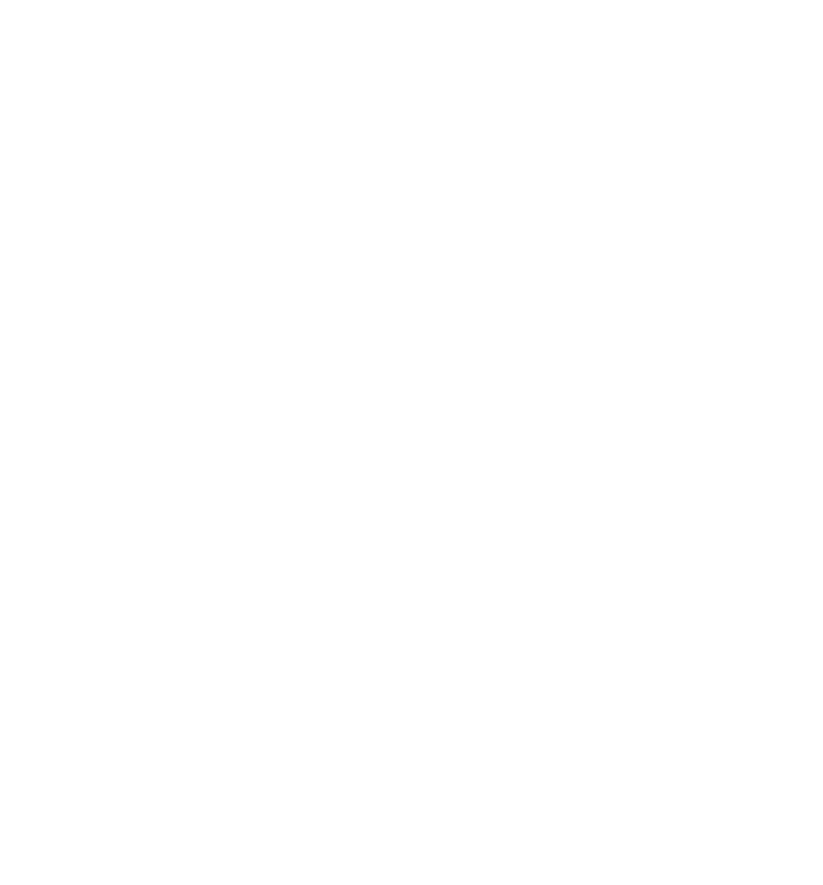
\includegraphics[width=\columnwidth]{./Img/Experiment11_scheme_oneReceiver.pdf}
	}}
	\caption[Scheme of basic scenario]{Scheme of basic scenario with one noise source and one point of measure}
	\label{oneReceiverOneNSScheme}
	\end{subfigure}
	\begin{subfigure}[c]{0.45\textwidth}
		\centering
		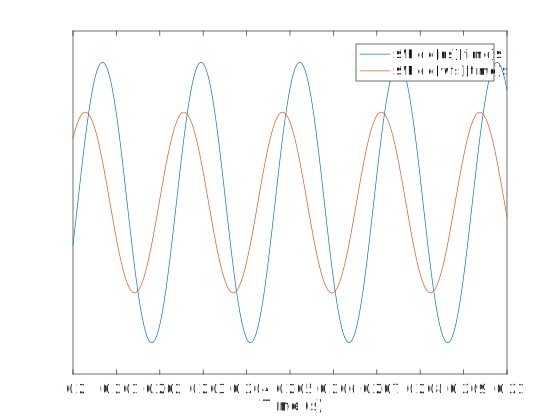
\includegraphics[width=\columnwidth]{Img/Experiment11_exampleNoFreqCorr.eps}
		\caption{Signal measured}
		\label{oneReceiverPureDeltaReceived}
	\end{subfigure}
	\caption{Simulation in simple scenario with one noise source and one point of measure}
\end{figure}

In order to quantify the performance, we will use the concept of attenuation. It is a frequency dependent parameter, defined as the power of the received signal at one point divided by the power of the signal received exclusively from the noise source. The inverse of the attenuation is the cancellation.

We will express them usually in dB:
\begin{gather}
\attenuation(f) = 10\log{\left\lvert\frac{\Field[wfs][frequency](f) + \Field[ns][frequency](f)}{\Field[ns][frequency](f)}\right\rvert^2}\quad\si{dB}\\
\cancellation(f) = -\attenuation(f)
\end{gather}
The maximum cancellation will happen when $\Field[ns][frequency] = -\Field[wfs][frequency]$.

Another useful parameter is what I call correction factor $\correctionFactor(f)$. It is conceived as the complex number by which loudspeakers signals $\signal[wfs][frequency]$ should be multiplied in order to achieve maximum cancellation:
\begin{equation}
\correctionFactor(f) = -\frac{\Field[ns][frequency](f)}{\Field[wfs][frequency](f)}
\end{equation}

In the previous case, the cancellation and corrections factors are $\cancellation = 3.6\si{dB}$ and $\correctionFactor = 1.1 e^{j40.3/360}$.

Since the aim of WFS is achieving cancellation over an wide area, it is reasonable to measure the field not in just one location, but in a grid of points, and the cancellation will vary from one to another. In that case, it is convenient come up with some way of describing the overall performance with just one value that takes in account the field at every point of measure. The concept of global attenuation can be used, defined as the overall total power divided by the overall measured power with the loudspeakers turned off:
\begin{gather}
\globalAttenuation(f) = 10 \log \left[\frac{\sum_m \abs{\Field[ns][frequency][scalar][m](f) + \Field[wfs][frequency][scalar][m](f)}^2}{\sum_m \abs{\Field[ns][frequency][scalar][m](f)}^2}\right] \quad \si{dB}
\\
\globalCancellation(f) = -\globalAttenuation(f)
\end{gather}

In the same way, the correction factor has a global equivalent, the global correction factor $\globalCorrectionFactor$, defined as the number that must be multiplied by the loudspeaker signals $\signal[wfs][frequency]$ in order to minimize the overall measured power.
\begin{equation}
\globalCorrectionFactor(f) = \argmin_{\psi} \norm{\psi \Field[wfs][frequency][vector] + \Field[ns][frequency][vector]}^2 = -\frac{\scalarProd{\Field[wfs][frequency][vector]}{\Field[ns][frequency][vector]}}{\norm{\Field[wfs][frequency][vector]}^2}
\end{equation}
where $\Field[wfs][frequency][vector] = [\Field[wfs][frequency][scalar][1],...,\Field[wfs][frequency][scalar][\numMeasPoints]]^T$ and $\Field[ns][frequency][vector] = [\Field[ns][frequency][scalar][1],...,\Field[ns][frequency][scalar][\numMeasPoints]]^T$.

So, instead of one point, now let's see what happens at a grid of points (\autoref{MultipleReceiverOneNSCanc}). It seems cancellation is bad at all of them. The global cancellation value is $\globalCancellation = 2.37 dB$. 

\begin{figure}
	\centering			\includegraphics[height=0.3\textheight]{./Img/Experiment11_multipleReceiverAtten2Dmap.eps}
	\caption[Attenuation 2D map]{Attenuation 2D map in dB}
	\label{MultipleReceiverOneNSCanc}
\end{figure}

It might be that the bad results have to do with the location of the noise source. Let's then see what happens for different positions as shown in \autoref{MultRecMultNSscheme}. Instead of just showing the 2D map of cancellations for each noise source positions, it will be more convenient for farther analysis to visualize it as a histogram of global cancellation values
\autoref{histogramDifNSNoFreqCorr}.

\begin{figure}
	\centering
	\begin{subfigure}[b]{0.49\textwidth}
	\centering
	\reflectbox{\rotatebox[origin=c]{180}{
			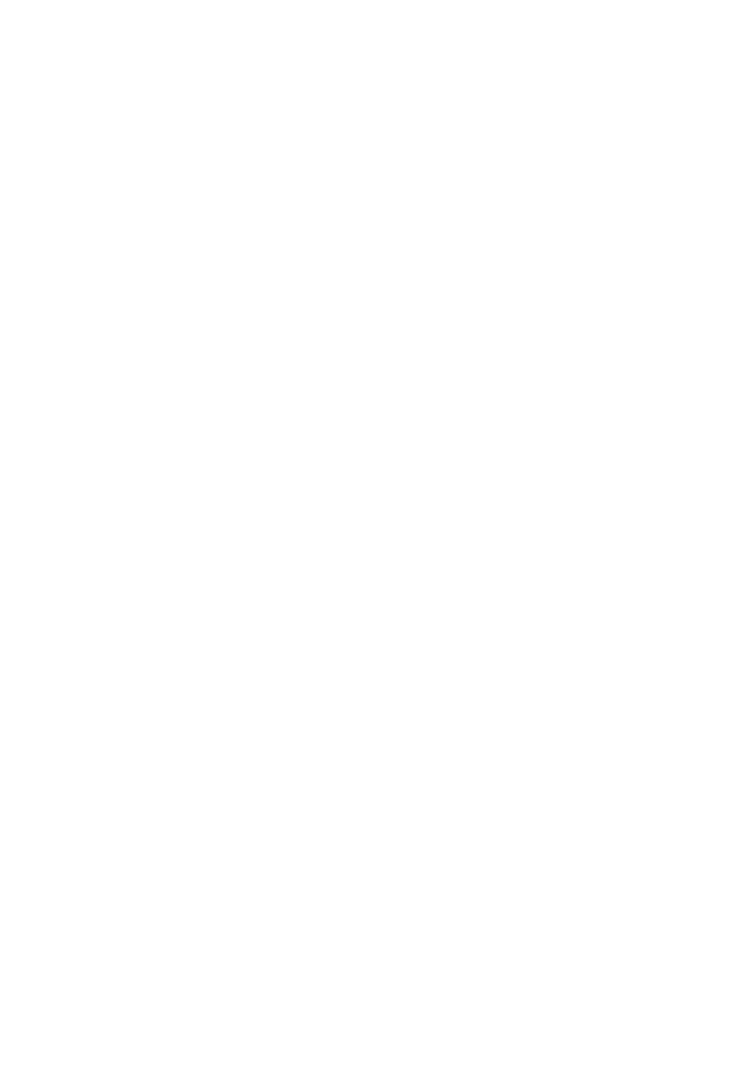
\includegraphics[height=0.3\textheight]{./Img/Experiment11_scheme_multipleReceiverMultipleNS.pdf}
	}}
	\caption[Scheme of multiple points of measure and multiple noise source positions]{Scheme of multiple points of measure and multiple noise source positions}
	\label{MultRecMultNSscheme}
	\end{subfigure}
	\begin{subfigure}[b]{0.49\textwidth}
	\centering
	\includegraphics[height=0.3\textheight]{./Img/Experiment11_attenGlobDifNSNoFreqCor.eps}
	\caption{Histogram of global cancellations}
	\label{histogramDifNSNoFreqCorr}
	\end{subfigure}
	\caption{Multiple positions of the noise source}
\end{figure}

However, all this has been tested just at one frequency. Maybe, the behaviour for the rest of frequencies is different. To check it out, we will make the noise source transmit a chirp signal from $20 \si{Hz}$ to $940 \si{Hz}$ (close to the aliasing spatial frequency) and then calculate the FFT\showto{private}{(for more information on how the simulations are carried out, consult appendix \autoref{appendixSimulation})}. The global cancellation for one noise source position is shown in \autoref{globCancOneNSchirp}. It is obvious that the values are bad over the whole bandwidth.

\begin{figure}[h]
	\centering
	\includegraphics[width=0.4\textwidth]{./Img/Experiment11_globalCancOneNSChirp.eps}
	\caption{Global attenuation for the whole bandwidth and a given noise source position}
	\label{globCancOneNSchirp}
\end{figure}

In order to understand what is happening for the whole bandwidth and multiple source position in just one snapshot, consider \autoref{histogram3D}. It is a histogram of global cancellations, similar to \autoref{histogramDifNSNoFreqCorr}, but seen in 3D, and each bar has been coloured according to the height. If we look at it from above (\autoref{histogram3Dabove}), we won't appreciate the heigh, but the colour will be enough.
That histogram is particularized for just one frequency ($440\si{Hz}$). If, for each frequency, we generate a similar coloured histogram and stack them next to each other, we can form an image as \autoref{histogramGlobAttenDifNS} where the x axis is the frequency, the y axis is the cancellation value, and the colour is the ratio of occurrences in that interval; in other words, each column is a histogram of values. The histogram tells us that the cancellation is bad at all frequencies, for every position of the noise source.

\begin{figure}[h]
	\centering
	\begin{subfigure}[b]{0.49\textwidth}
	\centering
	\includegraphics[width=0.8\textwidth]{./Img/Experiment11_attenGlobDifNSchirp3Dhist.eps}
	\caption{Example of global attenuation histogram in 3D}
	\label{histogram3D}
	\end{subfigure}
	\begin{subfigure}[b]{0.49\textwidth}
		\centering
		\includegraphics[width=0.8\textwidth]{./Img/Experiment11_attenGlobDifNSchirp3DhistAbove.eps}
		\caption{Example of global attenuation histogram in 3D seen from above}
		\label{histogram3Dabove}
	\end{subfigure}
	\begin{subfigure}[b]{0.49\textwidth}
		\centering	\includegraphics[width=0.8\textwidth]{./Img/Experiment11_DifNSchirpGlobAtten.eps}
		\caption{Completed global attenuation histogram}
		\label{histogramGlobAttenDifNS}
	\end{subfigure}
\caption{Frequency dependent histogram of attenuation, step by step}
\end{figure}

What is happening? The answer can be found if we represent the global correction factor $\globalCorrectionFactor$ (\autoref{GlobalCorrFact}). We can see that, even when there is some variance between the values for different noise source positions, the overall tendency follows the theoretical expression $\sqrt{jk/2\pi}$ that was omitted for being considered unnecessary. This result suggests that it is, indeed, necessary.

\begin{figure}[h]
	\begin{subfigure}[b]{0.49\textwidth}
		\centering
		\includegraphics[width=0.8\textwidth]{./Img/Experiment11_DifNSchirpGlobCorrFactAbs.eps}
		\caption{$|\globalCorrectionFactor|$}
		\label{GlobalCorrFactAbs}
	\end{subfigure}
	\begin{subfigure}[b]{0.49\textwidth}
		\centering
		\includegraphics[width=0.8\textwidth]{./Img/Experiment11_DifNSchirpGlobCorrFactPhase.eps}
		\caption{$\angle{\globalCorrectionFactor}$}
		\label{GlobalCorrFactPhase}
	\end{subfigure}
\caption{Global correction factor $\globalCorrectionFactor$}
\label{GlobalCorrFact}
\end{figure}

The reason for this is that, even though that term is expendable when generating wave fields that are going to be heard by humans, it is required when the aim is to interference destructively with another existing wave field. For example, for a noise field $\Field[ns][frequency] = 1$, the secondary source field should be $\Field[wfs][frequency] = -1$ for perfect cancellation $\attenuation = -\infty \si{dB}$. But if the phase is shifted $-\pi/4$ ($1/\sqrt{j} = e^{-j\pi/4}$), the amplitude of the field is $|\Field[ns][frequency] + \Field[wfs][frequency]| = |1 - e^{-j\pi/4}| = 0.77$, which corresponds to a cancellation of $\cancellation = 2.32\si{dB}$. Amplitude variations of course also worsen the cancellation levels. So, the term $\sqrt{jk/2\pi}$ might irrelevant when for the human ear when listening to a signal, but are of vital importance if we are going to make a cancelling wave physically interfere with another. We can't get away with just ignoring it.

In conclusion, a $\sqrt{jk/2\pi}$ filter must be implemented in WFS when the intention is to perform active cancellation of noise. Theoretically the filter has an anticausal response, but it must be implemented as a FIR digital filter, so inevitably it will introduce some amount of delay that must be compensated \cite{Lapini2018}. That sets a constraint on how close the noise source can be to the loudspeaker array, as we will see in next section.

\section{Compromise between frequency filter length and accuracy}

\begin{shownto}{private}
	Consultar \cite{FrankSchutz2015}
\end{shownto}

In previous section we've concluded that, in order to produce cancellation inside the area enclosed by the loudspeaker array, a filter with a frequency response $\sqrt{jk/2\pi} = \sqrt{jf/c}$ must be implemented in the form of a FIR digital filter. This has a drawback, and it is that the ideal theoretical filter is anticausal. This means that, in order to calculate the output signal $y$ at a time $t$, it needs to use input values that come after that time: $y(t)$ depends on $x(t+\Delta t)$, being $\Delta t > 0$. This is exactly like knowing the future. Mathematically speaking, that can make sense, and in simulations it isn't a limitation either since we know exactly what the noise source signal is going to be.
But in real-time systems it is, obviously, impossible to implement.

However, there is a nuance that can allow us to implement this filter in real-time. Let's complete \autoref{wfsSignalTime} with the new filter:
\begin{equation}
\begin{aligned}
\signal[wfs][time](t) &= \signal[nsVirt][time](t) \frac{g \cos\normPrimaryPropAngleSection}{\sqrt{\distLinePrimSource}}
\ast\delta(t - \distLinePrimSource/c)\ast h(t) = \signal[nsVirt][time](t) \frac{g \cos\normPrimaryPropAngleSection}{\sqrt{\distLinePrimSource}}
\ast h(t - \distLinePrimSource/c)\\
h(t) &= \FourierTransform{\sqrt{\frac{jk}{2\pi}}}[inverse]
\end{aligned}
\end{equation}

When we say that $h(t)$ is anticausal, it is the same as saying that there are negative values of $t$ for which $h(t) \neq 0$. As long at this doesn't change, the practical implementation of this filter won't be possible. Nonetheless, let's notice that the loudspeaker signal $\signal[wfs][time](t)$ doesn't depend directly on $\signal[nsVirt][time](t)$ filtered by $h(t)$, but on a delayed version of it: $h(t - \distLinePrimSource/c)$.

If the filter impulse response $h(t)$ was limited in time ($h(t) = 0, t < -\tau_1$), then, although $h(t)$ would be anticausal, $h(t - \distLinePrimSource/c)$ will be causal as long as $\distLinePrimSource/c > \tau_1$. However, since the ideal $h(t)$ has an infinite response, the only option left is to use an approximation ($\widetilde{h}(t)$) that satisfies that $\widetilde{h}(t) = 0$ for $t < -\tau_1$, where $\tau_1 < \distLinePrimSource/c$. The delayed filter $\widetilde{h}(t - \distLinePrimSource/c)$ is causal, and hence could work in a real time system.

If, in addition, it has a finite duration, it would be implementable as a FIR digital filter. This means it must satisfy that $h(t) = 0, t \notin [-\tau_1, \tau_2]$. Matlab has its own internal functions to design FIR filters based on their frequency response, and in general returns impulse responses where $\tau_1 = \tau_2 = \tau$. However, as it works as an approximation, the smaller $\distLinePrimSource/c$ gets, the shorter the duration of the impulse response needs to be, and hence the worse the approximation and the accuracy of WFS will be. So, there is actually a trade-off between performance and the distance between the source and the closest loudspeaker $\distLinePrimSource$. The smaller the distance, the worse the performance. At a given sampling frequency, which is $44100 \si{Hz}$ in our simulations, the duration of the impulse response translates directly to number of coefficients of the digital filter.

We should differentiate between the filter that implements the magnitude of the frequency response $h_1 = \sqrt{f/c}$ and the one that implements the frequency independent phase shift $h_2 = \sqrt{j}$, because they present different requirements. The real implementations will be called $\widetilde{h}_1$ and $\widetilde{h}_2$ respectively.

We have plotted the histograms of attenuation for different lengths of the implementation of $\widetilde{h}_1$ (\autoref{globCancDifMagFilterLength}), keeping $\widetilde{h}_2$ with a high enough length so it resembles the ideal case and doesn't produce any noticeable distortion. We can see that, below an order of $64$ (the order of a FIR filter is its length minus 1), the performance starts to get worse and worse. Above it, the improvement is not too noticeable.
\begin{figure}[h]
	\centering
	\begin{subfigure}[b]{0.45\textwidth}
		\centering
		\includegraphics[width=\columnwidth]{../TFM/Img/Experiment12_globalAttenMagnOrder_8.eps}
		\caption{Order: $8$. $\tau = 0.091 \si{ms}$. ${\distLinePrimSource}_{min} = 3\si{cm}$}
	\end{subfigure}
	\begin{subfigure}[b]{0.45\textwidth}
		\centering
		\includegraphics[width=\columnwidth]{../TFM/Img/Experiment12_globalAttenMagnOrder_16.eps}
		\caption{Order: $16$. $\tau = 0.181 \si{ms}$. ${\distLinePrimSource}_{min} = 6\si{cm}$}
	\end{subfigure}
	\begin{subfigure}[b]{0.45\textwidth}
		\centering
		\includegraphics[width=\columnwidth]{../TFM/Img/Experiment12_globalAttenMagnOrder_32.eps}
		\caption{Order: $32$. $\tau = 0.363 \si{ms}$. ${\distLinePrimSource}_{min} = 12\si{cm}$}
	\end{subfigure}
	\begin{subfigure}[b]{0.45\textwidth}
		\centering
		\includegraphics[width=\columnwidth]{../TFM/Img/Experiment12_globalAttenMagnOrder_64.eps}
		\caption{Order: $64$. $\tau = 0.726 \si{ms}$. ${\distLinePrimSource}_{min} = 25\si{cm}$}
	\end{subfigure}
	
	\caption{Global attenuation for different lengths of $h_1$}
	\label{globCancDifMagFilterLength}
\end{figure}

We've done the same with $h_2 = \sqrt{j}$. In this case, a Hilbert filter must be implemented and, as we see in (\autoref{globCancDifHilFilterLength}), its length has to be much bigger than with the magnitude filter. $\widetilde{h}_1$ order is high enough so produced distortions are negligible. As can be observed, the order of $\widetilde{h}_2$ has to be much bigger than the order of $\widetilde{h}_1$, and it entails a more severe constraint. Orders of $4096$ and above get practically the same levels of attenuation, so it makes no sense to go beyond $4096$. However, such a long filter implies that the distance from the noise source to the closest loudspeaker should be at least $15.79 \si{m}$, a restriction that can't always be met.

\begin{figure}[h]
	\centering
	\begin{subfigure}[b]{0.45\textwidth}
		\centering
		\includegraphics[width=\columnwidth]{../TFM/Img/Experiment12_globalAttenHilbOrder_512.eps}
		\caption{Order: $512$. $\tau = 5.8 \si{ms}$. ${\distLinePrimSource}_{min} = 1.97\si{m}$}
	\end{subfigure}
	\begin{subfigure}[b]{0.45\textwidth}
		\centering
		\includegraphics[width=\columnwidth]{../TFM/Img/Experiment12_globalAttenHilbOrder_1024.eps}
		\caption{Order: $1024$. $\tau = 11.6 \si{ms}$. ${\distLinePrimSource}_{min} = 3.95\si{m}$}
	\end{subfigure}
	\begin{subfigure}[b]{0.45\textwidth}
		\centering
		\includegraphics[width=\columnwidth]{../TFM/Img/Experiment12_globalAttenHilbOrder_2048.eps}
		\caption{Order: $2048$. $\tau = 23.2 \si{ms}$. ${\distLinePrimSource}_{min} = 7.89\si{m}$}
	\end{subfigure}
	\begin{subfigure}[b]{0.45\textwidth}
		\centering
		\includegraphics[width=\columnwidth]{../TFM/Img/Experiment12_globalAttenHilbOrder_4096.eps}
		\caption{Order: $4096$. $\tau = 46.4 \si{ms}$. ${\distLinePrimSource}_{min} = 15.79\si{m}$}
	\end{subfigure}
	
	\caption{Global attenuation for different lengths of $h_2$}
	\label{globCancDifHilFilterLength}
\end{figure}

\showto{private}{
\subsection{Alternatives}}

\begin{shownto}{private} % Needs to be completed
\section{Performance in non-free-space conditions}
Every simulation that has been done so far has assumed free-space conditions. However, in a real set-up there are all kinds of reflections, diffraction effects, etc. Simulations of more real conditions are interesting. In order to do so, a Room Impulse Response generator was used. It has been developed by International Audio Laboratories Erlangen \cite{RIRgenerator}. It allows to define the dimensions of a room in the shape of a rectangular box ($[x,y,z]$), the reflection coefficients of each one of the six walls, and calculate, using the image method, the impulse responses between points specified by the user. Those impulse responses have been used instead of the free space ones.

The order of the filters $\widetilde{h}_1$ and $\widetilde{h}_2$ are high enough so they don't cause any relevant inaccuracies. The same reflection coefficient $\reflectCoef$ has been used for every wall. The room dimensions have been choosen to fit in every noise source: $[8, 11.2, 4]\si{m}$, and all sources, loudspeakers and receiving points have a height of $1.65\si{m}$ (\autoref{roomDimFig}).

\begin{figure}
	\centering
	\fbox{
	\reflectbox{\rotatebox[origin=c]{180}{
			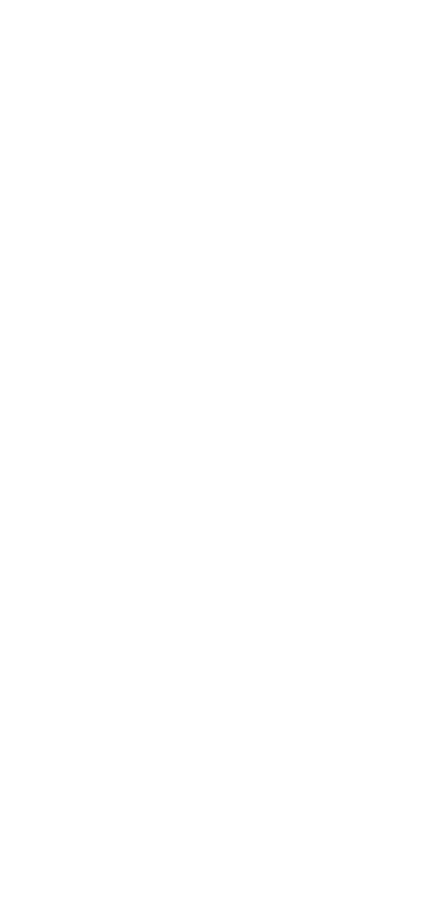
\includegraphics[height=0.3\textheight]{./Img/Experiment13_scheme.pdf}
	}}
}
\caption{Scheme of the simulated room}
\label{roomDimFig}
\end{figure}

\autoref{globAttenDifReflectCoef} shows the attenuation histogram for different values of $\reflectCoef$. When it goes above $0.2$, cancellation levels drop down below $10 \si{dB}$.

\begin{figure}[h]
	\centering
	\begin{subfigure}[b]{0.45\textwidth}
		\centering
		\includegraphics[width=\columnwidth]{../TFM/Img/Experiment13_globalAttenReflCoef_0.eps}
		\caption{$\beta = 0$}
	\end{subfigure}
	\begin{subfigure}[b]{0.45\textwidth}
		\centering
		\includegraphics[width=\columnwidth]{../TFM/Img/Experiment13_globalAttenReflCoef_10.eps}
		\caption{$\beta = 0.25$}
	\end{subfigure}
	\begin{subfigure}[b]{0.45\textwidth}
		\centering
		\includegraphics[width=\columnwidth]{../TFM/Img/Experiment13_globalAttenReflCoef_20.eps}
		\caption{$\beta = 0.5$}
	\end{subfigure}
	\begin{subfigure}[b]{0.45\textwidth}
		\centering
		\includegraphics[width=\columnwidth]{../TFM/Img/Experiment13_globalAttenReflCoef_50.eps}
		\caption{$\beta = 0.75$}
	\end{subfigure}
	
	\caption{Global attenuation for different reflection coefficients $\reflectCoef$}
	\label{globAttenDifReflectCoef}
\end{figure}

\subsection{GTAC anechoic chamber}
The impulse responses from the anechoic chamber were measured...
From the relation of distance and magnitude of the impulse response, we can suggest that the reflection coefficient is equivalent to...
\end{shownto}

\section{Truncation and lower cut-off frequency} % Experiment10.m
There is a remarkable phenomenon that can be observed through all simulations. If we take a look at any of the previously shown attenuation histograms, we will see that from approximately $200\si{Hz}$ down, the performance gets poorer as the frequency decreases. It is as if the system had a lower cut-off frequency of $200\si{Hz}$ below which it doesn't work properly (\autoref{lowCutOffFreqExample}). That transition region is there due to the fact that in practice, the line of secondary sources (the loudspeaker array) has a finite length, in other words, it is truncated. In order to explain this, it is convenient to recall some of the theoretical expressions of WFS.

\begin{figure}[h]
\centering
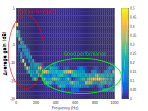
\includegraphics[width=0.5\columnwidth]{../TFM/Img/LowCutoffFrequencyDegradationExample.pdf}
\caption{Example of performance degradation for low frequencies}
\label{lowCutOffFreqExample}
\end{figure}

As we've already seen, the field created by a monopole source (primary source) located at $\PosTheo[primarySource]$ at a receiving point $\PosTheo$ is:
\begin{equation}
\Field[primarySource](\PosTheo) = \CoefTheo[primarySource](f)  \frac{e^{-jk\norm{\PosTheo - \PosTheo[primarySource]}}}{\norm{\PosTheo - \PosTheo[primarySource]}}
\end{equation}
where $f$ is the frequency, $\CoefTheo[primarySource](f)$ is the feeding coefficient to the source, and $k = \frac{2\pi}{\lambda}$ is the propagation constant.

Rayleigh I 2.5D integral allows to replicate the field by an infinite line distribution of monopole sources (secondary sources), given the condition that all points where the field is replicated, as well as the primary source location and the secondary source line distribution ($\sectionTheo$), are all on the same plane, and that the secondary source line separates the reconstructed field region from the primary source. The expression is:
\begin{equation}
\begin{aligned}
\Field(\PosTheo) &= \int_{\sectionTheo} \CoefTheo[section][monopole][rayleigh](\PosTheo[section], \PosTheo) \frac{e^{-jk\distLinePoint}}{\distLinePoint} \mathrm{d}\PosTheo[section]\\
\CoefTheo[section][monopole][rayleigh](\PosTheo[section]) &= \CoefTheo[primarySource] \cos\normPrimaryPropAngleSection \frac{e^{-jk\distLinePrimSource}}{\sqrt{\distLinePrimSource}} \sqrt{\frac{jk}{2\pi}} \sqrt{\frac{d}{d + d_{\PosTheoSubInd[primarySource]}}}
\end{aligned}
\end{equation}
where $Q(\PosTheo[section], \PosTheo)$ is the feeding of the differential secondary monopole source located at $\PosTheo[section]$, $\distLinePrimSource = \norm{\PosTheo[section] - \PosTheo[primarySource]}$ is the distance from the primary source to the secondary source and $\distLinePoint = \norm{\PosTheo[section] - \PosTheo}$ is the distance from the secondary source to the reconstruction point and $d_{\PosTheoSubInd[primarySource]}$ is the distance between the primary source and the secondary source line. It is valid for values of $k\distLinePrimSource >> 1$. The field is replicated with correct amplitude over a line parallel to the secondary source line and separated a distance $d$.

One of the reasons why Rayleigh I 2.5D integral is still far from practical applications is that the line distribution of monopoles $\sectionTheo$ has an infinite longitude, which is of course unrealistic. At some point the line has to be truncated, and hence, the accuracy of the reconstructed field will be affected.

In order to study this limitation, we can look at a simple scenario where a line of secondary sources $\sectionTheoLength$ meters long is located at the x axis from from $-\sectionTheoLength/2$ to $\sectionTheoLength/2$, a primary source is located on the negative y axis at $\PosTheo[primarySource] = [0, -d_{\PosTheoSubInd[primarySource]}, 0]$ and the receiving point on the positive y axis at $\PosTheo = [0, d, 0]$ (\autoref{truncationScheme}). Depending on those four parameters, three distances ($\sectionTheoLength$, $d_{\PosTheoSubInd[primarySource]}$ and $d$) plus the frequency $f$, the accuracy of the synthesized field will vary.

\begin{figure}[h]
	\centering
	\def\svgwidth{0.5\columnwidth}
	\graphicspath{{../TFM/Img/}}
	\input{../TFM/Img/Experiment10_truncationScheme.pdf_tex}
	\caption{Scheme of truncation scenario}
	\label{truncationScheme}
\end{figure}

In this scenario, the reconstructed field at point $\PosTheo$ is:
\begin{equation}
\Field(\PosTheo) = \int_{-\sectionTheoLength/2}^{\sectionTheoLength/2} \CoefTheo[section][monopole][rayleigh](\PosTheo[section][x], \PosTheo) \frac{e^{-jk\distLinePoint}}{\distLinePoint} \mathrm{d}\PosTheo[section][x]
\label{Rayleigh2_5DTruncatedIntegral}
\end{equation}
where $\distLinePrimSource = \norm{\PosTheo[section] - \PosTheo[primarySource]} = (d_{\PosTheoSubInd[primarySource]}^2 + \PosTheo[section][x]^2)^{1/2}$ is the distance from the primary source to the secondary source, $\distLinePoint = \norm{\PosTheo[section] - \PosTheo} = (d^2 + \PosTheo[section][x]^2)^{1/2}$ is the distance from the secondary source to the reconstruction point and $\cos\normPrimaryPropAngleSection = d_{\PosTheoSubInd[primarySource]}/\distLinePrimSource$ is the cosine of the angle of incidence.

A useful measure that facilitate the evaluation of the accuracy is the relative field $\Field_\mathit{rel}(\PosTheo)$, this is, the resulting field divided by the ideal one produced by the primary source.
\begin{equation}
	\Field_\mathit{rel}(\PosTheo) = \frac{\Field(\PosTheo)}{\Field[primarySource](\PosTheo)}
\end{equation}
The closer $\Field_\mathit{rel}$ is to $1$ the better the accuracy. The starting point will be a very simple case, and then we will add some complexity.

\begin{shownto}{private}
This measure depend on the spatial parameters of the scenario (position of primary source $\PosTheo[primarySource]$, shape and location of the second source line distribution $\sectionTheo$, and location of the receiving point $\PosTheo$) and the wavelength $\lambda$. However, if we scale all parameters by a factor $C$ ($\PosTheo[primarySource]^{(s)} = C \PosTheo[primarySource]$, $\PosTheo^{(s)} = C\PosTheo$, $\PosTheo[section]^{(s)} = C\PosTheo[section]$, $\lambda^{(s)} = C\lambda$) and recalculate the signal of each secondary source, the relative field will be exactly the same due to the properties of the integral. This fact is useful because allows to, for example, express all distances in wavelengths ($d^{(s)} = d/\lambda$, $d_{\PosTheoSubInd[primarySource]}^{(s)} = d_{\PosTheoSubInd[primarySource]}/\lambda$, $L^{(s)} = L/\lambda$) and fixate the wavelength to $1$ ($\lambda = 1$), reducing the number of variables from four to three.
\end{shownto}

\subsection{Ideal case: $\sectionTheoLength=\infty$}
First, we consider an array of infinite length $\sectionTheoLength=\infty$.
% where each monopole secondary source transmits a signal $Q_\mathit{perfect}$:
%\begin{equation}
%Q_\mathit{perfect}(\PosTheo[section], \PosTheo) = \cos\normPrimaryPropAngleSection \frac{e^{-jk\distLinePrimSource}}{\sqrt{\distLinePrimSource}} \left(\sqrt{\frac{j k}{2\pi}} + \frac{1}{\distLinePrimSource \sqrt{j 2 \pi k}}\right) \sqrt{\frac{\distLinePoint}{\distLinePrimSource + \distLinePoint}}
%\end{equation}
Theoretically, any inexactitude must necessarily be produced by the application of the stationary point method in the dimensionality reduction from a plane to a line, and to the assumption that the primary source is in the far field $k\distLinePrimSource >> 1$ (\autoref{chapterWFStheory}).

In numerical calculation of the integral in Matlab (\autoref{TruncIdealRecFarPSclose}) shows that when $d_{\PosTheoSubInd[primarySource]}$ gets smaller, the reconstructed field deteriorates, and so WFS is actually not useful under such conditions. A similar behaviour but much less severe is found when the primary source is in the far field but the receiving point is very near the secondary source line (\autoref{TruncIdealPSFarRecClose}).
\begin{figure}[h]
	\centering
	\begin{subfigure}[b]{0.49\textwidth}
		\centering
		\includegraphics[width=0.9\textwidth]{Img/Experiment10_TruncationIdealCaseA.eps}
		\caption{$d/\lambda \gg 1$}
		\label{TruncIdealRecFarPSclose}
	\end{subfigure}
	\begin{subfigure}[b]{0.49\textwidth}
		\centering
		\includegraphics[width=0.9\textwidth]{Img/Experiment10_TruncationIdealCaseB.eps}
		\caption{$d_{\PosTheoSubInd[primarySource]}/\lambda \gg 1$}
		\label{TruncIdealPSFarRecClose}
	\end{subfigure}
	\caption{Magnitude and phase of the relative field for an infinite line array $\sectionTheoLength = \infty$}
\end{figure}
In conclusion, as long as both the primary source and the receiving point are not too close to the secondary source line, the precision won't be too distorted.

\subsection{Primary source in the infinite}
Let's take the case where the primary source is far: $d_{\PosTheoSubInd[primarySource]} \gg 1$. Then,
\begin{gather*}
	\cos\normPrimaryPropAngleSection \approx 1 \\ \distLinePrimSource \approx d \\ \sqrt{\frac{d}{d_{\PosTheoSubInd[primarySource]} + d}} \approx \sqrt{\frac{d}{d_{\PosTheoSubInd[primarySource]}}}
\end{gather*}
for all the segment $\PosTheo[section][x] \in [-\sectionTheoLength/2, \sectionTheoLength/2]$, so \autoref{Rayleigh2_5DTruncatedIntegral} simplifies to:
\begin{multline}
	P(\PosTheo) = \int_{-\sectionTheoLength/2}^{\sectionTheoLength/2} Q(x_{\PosTheoSubInd[section]}, \PosTheo) \frac{e^{-jk\distLinePoint}}{\distLinePoint} \mathrm{d}\PosTheo[section][x] =\\
	= \left\{Q(x_{\PosTheoSubInd[section]}, \PosTheo) =  \frac{e^{-jkd_{\PosTheoSubInd[primarySource]}}}{\sqrt{d_{\PosTheoSubInd[primarySource]}}} \sqrt{\frac{j k}{2\pi}} \sqrt{\frac{d}{d_{\PosTheoSubInd[primarySource]}}}\right\} = \\
	= \frac{e^{-jkd_{\PosTheoSubInd[primarySource]}}}{\sqrt{d_{\PosTheoSubInd[primarySource]}}} \sqrt{\frac{j k}{2\pi}} \sqrt{\frac{d}{d_{\PosTheoSubInd[primarySource]}}} \int_{-\sectionTheoLength/2}^{\sectionTheoLength/2} \frac{e^{-jk\distLinePoint}}{\distLinePoint} \mathrm{d}\PosTheo[section][x]
	\label{truncDeductionI}
\end{multline}

The integral is actually the field generated by a linear source. When we are dealing with an infinite line source ($\sectionTheoLength \to \infty$), the exact solution is a scaled version of the zero-th order of the Hankel function of second type. Nonetheless it approximates very well to another much more useful expression:
\begin{equation}
\int_{-\infty}^{\infty} \frac{e^{-jk\distLinePoint}}{\distLinePoint} \mathrm{d}x_{\PosTheoSubInd[section]} = -\pi j \mathrm{H_0^{(2)}(k d)} \approx \frac{e^{-jkd}}{\sqrt{kd}}\sqrt{\frac{2\pi}{j}}
\label{fieldLinearSource}
\end{equation}

Substituting \autoref{fieldLinearSource} in \autoref{truncDeductionI}:
\begin{equation}
P(\PosTheo) \approx \frac{e^{-jkd_{\PosTheoSubInd[primarySource]}}}{\sqrt{d_{\PosTheoSubInd[primarySource]}}} \sqrt{\frac{j k}{2\pi}} \sqrt{\frac{d}{d_{\PosTheoSubInd[primarySource]}}} \frac{e^{-jkd}}{\sqrt{kd}}\sqrt{\frac{2\pi}{j}} = \frac{e^{-jk(d_{\PosTheoSubInd[primarySource]} + d)}}{d_{\PosTheoSubInd[primarySource]}} \approx \frac{e^{-jk(d_{\PosTheoSubInd[primarySource]} + d)}}{d_{\PosTheoSubInd[primarySource]} + d} = P_{\PosTheoSubInd[primarySource]}(\PosTheo)
\end{equation}

So, when $\sectionTheoLength \to \infty$, the synthesized field is the same as the field from the primary source, as stated by WFS theory. What happens when the length of the secondary source line gets shorter? It all comes dowm to the integral:
\begin{equation}
I(\lambda/\sectionTheoLength, d/\sectionTheoLength) = \int_{-\sectionTheoLength/2}^{\sectionTheoLength/2} \frac{e^{-jk\distLinePoint}}{\distLinePoint} \mathrm{d}\PosTheo[section][x] = \int_{-1/2}^{1/2} \frac{e^{-j\frac{2\pi}{\lambda/\sectionTheoLength}\sqrt{(d/\sectionTheoLength)^2 + \PosTheo[section][x]^2}}}{\sqrt{(d/\sectionTheoLength)^2 + \PosTheo[section][x]^2}} \mathrm{d}\PosTheo[section][x]
\label{lineSourceIntegralLfinite}
\end{equation}

\autoref{lineSourceIntegral} shows an example of how the integral evolves when increasing $\sectionTheoLength$. As we see, the magnitude and the phase oscillate and converges towards the value in \autoref{fieldLinearSource} when $\sectionTheoLength$ increases. It is pretty obvious that there is a transition period where $\sectionTheoLength$ is too small to produce accurate enough results.

\begin{figure}[h]
	\centering
	\includegraphics[width=0.4\textwidth]{Img/lineSourceIntegral.eps}
	\caption{Field generated by a linear source of length $L$ ($d = 10$, $k = 1$)}
	\label{lineSourceIntegral}
\end{figure}

As we've seen in \autoref{lineSourceIntegralLfinite}, $I$ depends actually just on $d/\sectionTheoLength$ and $\sectionTheoLength/\lambda$. In \autoref{lineSourceIntegralNorm} we've represented the value of $\sectionTheoLength/\lambda$ where the phase (and also the magnitude) starts to converge.

\begin{figure}[h]
	\centering
	\includegraphics[width=0.4\textwidth]{Img/LnormThreshold.eps}
	\caption{Minimum value of $\sectionTheoLength/\lambda$ where the value of $I$ (\autoref{lineSourceIntegralLfinite}) starts to converge}
	\label{lineSourceIntegralNorm}
\end{figure}

All this means that there is a lower cutoff frequency below which WFS is not useful. For example, \autoref{linseSourceIntegralGTAC} shows the cutoff frequency for a linear array of length $\sectionTheoLength = 0.18\cdot23 = 4.14\si{m}$, as one of the sides of the loudspeaker array in the GTAC anechoic chamber.
\begin{figure}[h]
	\centering
	\includegraphics[width=0.4\textwidth]{Img/freqThresholdGTAC.eps}
	\caption{Cutoff frequency for a linear array whose length is $\sectionTheoLength = 0.18\cdot23$, as two of the sides of the loudspeaker array in the GTAC anechoic chamber}
	\label{linseSourceIntegralGTAC}
\end{figure}

It's worth noticing that this analysis is done with a geometrically very simple scenario where the primary source is in the infinite, the receiving point is centred with respect to the secondary source line, we don't use complicated geometries as octagons, etc. The more variations we add, the more complex the results are. However, given what we observed in the simulations of the GTAC scenario, the existence of a lower cut-off frequency seems to be maintained even in those more complicated cases.

A deeper theoretical analysis of the truncation artefacts can be found in \cite[Section 4.3]{Start1997}, where various analytical approximations are proposed.

\begin{shownto}{private}
\section{Sampling frequency influence}
\end{shownto}